 \documentclass[11pt, oneside]{article} 
\usepackage{geometry}
\geometry{letterpaper} 
\usepackage{graphicx}
	
\usepackage{amssymb}
\usepackage{amsmath}
\usepackage{parskip}
\usepackage{color}
\usepackage{hyperref}

\graphicspath{{/Users/telliott_admin/Tex/png/}}
% \begin{center} 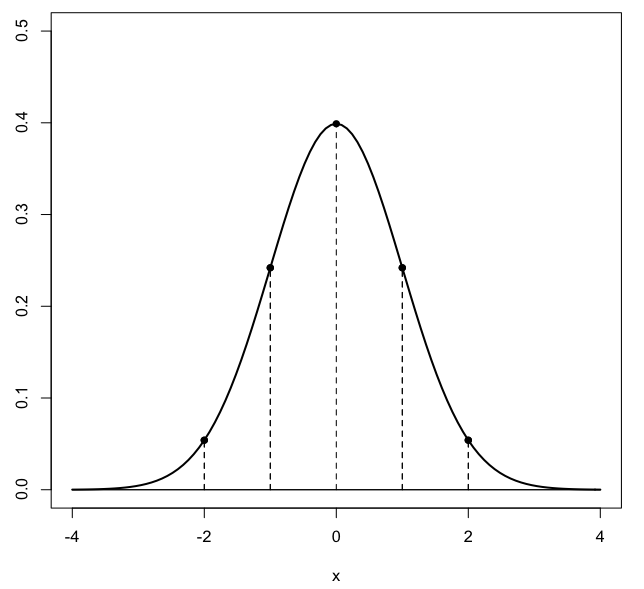
\includegraphics [scale=0.4] {gauss3.png} \end{center}

\title{Uniform circular motion}
\date{}

\begin{document}
\maketitle
\Large

\label{sec:Uniform_circular_motion}

Here we want to think about some problems related to the orbits of planets.  The first topic is uniform circular motion.  In this analysis we will idealize the orbits of the planets as circles.

The eccentricity of an ellipse is defined so that
\[ ea = f  \] 
where $f = \sqrt{a^2 - b^2}$ is the distance from the center to either focus.  If $e = 0$ then the curve is a circle rather than an ellipse.

According to wikipedia, the eccentricity of orbit of the objects known to Kepler (6 planets plus the moon) are
\[ 
\begin{array}{lcr}
\mbox{Mercury} & 0.024  \\
\mbox{Venus} & 0.007  \\
\mbox{Earth} & 0.017  \\
\mbox{Mars} & 0.093  \\
\mbox{Jupiter} & 0.048  \\
\mbox{Saturn} & 0.054  \\
\mbox{Moon} & 0.055  \\
\end{array}
\] 
These vary with time.

Looking at Earth, the distance from the sun is very nearly $150 \times 10^6$ km ($147,098,074$ at perihelion and $152,097,701$ km at aphelion, with a mean value of $149.6 \times 10^6$ km).

That is plus or minus $2.5 \times 10^6$ km or about $200$ earth diameters.

Besides the eccentricity of the orbit, there is also the complication that the earth does not "revolve around the sun" but instead both earth and sun revolve around their common center of mass. 

However the mass of the sun is about  $1.989 \times 10^{30}$ kg, while that of the earth is only about $5.972 \times 10^{24}$ kg.  The ratio is about $3.3 \times 10^5$.

So the center of mass is displaced from the center of the sun by about 
\[ \frac{5.972 \times 10^{24}}{1.989 \times 10^{30}} \ 150 \times 10^6 \approx 450 \]
That's $450$ km.  Since the sun's radius is about $695,000$ km, the center of mass is very close to the center of the sun.

\subsection*{basic equations}
We should be quite familiar with polar coordinates, we write
\[ x = R \cos \theta \]
\[ y = R \sin \theta \]
(I'm going to use $R$ for the radius since it's a constant in this analysis.  Also, we will also have $\mathbf{r}(t)$, the position vector).

We are talking about objects that change position with time, so we need to introduce time here somehow.  We will say that 
\[ \theta = \omega t \]
Our clock ticks in seconds, and $\omega$ (in units of radians per second) tells how $\theta$ is calibrated with respect to the clock.

So now we can write the components of 
\[ \mathbf{r}(t) = \langle \ x(t), y(t) \ \rangle \]
\[ = R \ \langle \cos \theta, \sin \theta \rangle \]
\[ = R \ \langle \cos \omega t, \sin \omega t \rangle \]
We have the magnitude $R$ times a unit vector.

And then we just differentiate to find the velocity and acceleration
\[ \mathbf{r}(t) = R \ \langle \cos \omega t, \sin \omega t \rangle \]
\[ \mathbf{v}(t) = \omega R \ \langle -\sin \omega t, \cos \omega t \rangle \]
\[ \mathbf{a}(t) = -\omega^2 R \ \langle \cos \omega t, \sin \omega t \rangle \]
\[ = -\omega^2 R \ \mathbf{r}(t) \]

Notice that $\mathbf{v}(t)$ is orthogonal to $\mathbf{r}(t)$ (compute the dot product to see this)
\[ \mathbf{v}(t) \cdot \mathbf{r}(t) = 0 \]

\begin{center} 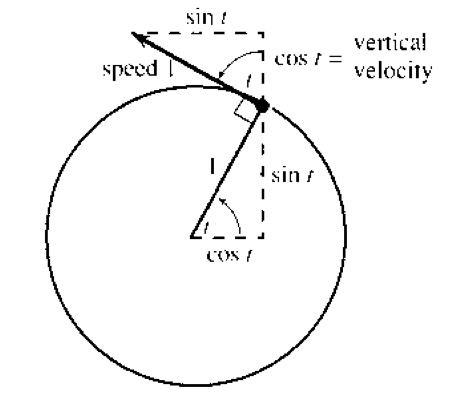
\includegraphics [scale=0.5] {strang_ucm.png} \end{center}
and the acceleration is on exactly the same line as $\mathbf{r}$ but points inward, toward the sun or origin of the system.
\[ \mathbf{a}(t) = -\omega^2 R \ \mathbf{r}(t) \]

Perhaps if we adjusted our clock to have the appropriate units of time, we wouldn't need $\omega$, but it gives the magnitude of the velocity.
\[ v = |\mathbf{v}| \]
\[ = | \omega R \ \langle -\sin \omega t, \cos \omega t \rangle | \]
\[ = \sqrt{\omega^2 R^2 (\sin^2  \omega t + \cos^2  \omega t)} \]
\[ = \sqrt{\omega^2 R^2 (\sin^2  \theta + \cos^2  \theta)} \]
\[ = \omega R  \]
and
\[ a = |\mathbf{a}| = \omega^2 R \]

We combine these to get an important identity
\[ a =  \omega^2 R = (\frac{v}{R})^2 R = \frac{v^2}{R} \]
\[ aR = v^2 \]
\[ v = \sqrt{aR} \]

We can apply the formula to find the orbital velocity for an object going around the earth.  The acceleration due to gravity is 
\[ a = \frac{GM}{R^2} \]
and then the orbital velocity is
\[ v = \sqrt{aR} = \sqrt{\frac{GM}{R}} \]

So called low-earth orbits start at a height of about $160$ km.  We add that to the earth's radius ($6371$ km)
\[ v = \sqrt{aR}  = \sqrt{0.0098 \cdot 6531} = 8.00 \]
in kilometers per second.

Compare this to the radial velocity at earth's equator which is about
\[ 40075 / (24 \cdot 3600) = 4.63 \]
in km per second.  There's a reason why rockets are launched from Florida.

Of course, the radial velocity depends on latitude.  One must multiply by the cosine of the latitude.  The radial velocity at the north pole is zero.

In addition to the energy from the orbital velocity, we also need to add the potential energy to get to a particular orbit.   We showed previously that
\[ V = - GM/R \]
\[ \Delta V = -GM(\frac{1}{R_2} - \frac{1}{R_1}) = GM(\frac{1}{R_1} - \frac{1}{R_2})\]

We can use these to look at some other orbits.
Geostationary orbit  42,000 km
Moon orbit avg = 385,000 km

The variation in satellite orbits is pretty extreme.

\subsection*{energy}
We did this calculation in the previous chapter.

The force due to gravity is
\[ \mathbf{F} = -\frac{GmM}{r^2} \hat{\mathbf{r}} \]
The potential is a function, which when we take
\[ - \frac{d}{dr} U = \mathbf{F} \]
\[ U = - \frac{GmM}{r} + C \]
Define
\[ U_{\infty} = 0 \rightarrow C = 0 \]
The total energy is
\[ E = K + U = \frac{1}{2}mv^2 - \frac{GmM}{r} \]
if we want an object to just reach $r=\infty$ with zero energy, starting from $r = R$, then
\[ 0 = \frac{1}{2}mv^2 - \frac{GmM}{R} \]
\[ v^2 = \frac{2GM}{R} \]
This is the escape velocity.

If the force is as given above, the magnitude of the acceleration is 
\[ a = \frac{GM}{r^2} \]
but for uniform circular motion we had
\[ a = \frac{v^2}{r} = \frac{GM}{r^2} \]
\[ v^2 = \frac{GM}{r} \]
or at the surface of the earth
\[ v^2 = \frac{GM}{R} \]
This is the orbital velocity.

So, near the earth's surface, the escape velocity is approximately $\sqrt{2}$ times the orbital velocity.

Finally, we know that the velocity is distance divided by time, so for one full revolution it is
\[ v = \frac{2\pi R}{T} \]
but
\[ v^2 = \frac{GM}{R} = (\frac{2\pi R}{T})^2 \]
Rearranging
\[ T^2 = \frac{(2\pi)^2}{GM} R^3 \]
This is Kepler's Third Law:  the square of the period is proportional to the cube of the orbit's radius.

The derivation is easy if we assume the orbits are circles, which is pretty close to being true.  It is also true for an elliptical orbit.  That is a bit harder calculation, which we will get to later.

\end{document}  